\documentclass[letterpaper,twocolumn,10pt]{article}

\usepackage[utf8]{inputenc}
\usepackage{usenix}
\usepackage[top=2cm,bottom=2.5cm,left=2cm,right=2cm]{geometry}
\usepackage{balance}
\usepackage{tikz}
\usepackage{xspace} % For reasonable spacing in custom commands.
\usepackage{xcolor} % For colourful links.
\usepackage[backend=biber,backref=true,maxnames=20,urldate=long]{biblatex}
\usepackage{hyperref} % For clickable links.
\usepackage[l2tabu, orthodox]{nag}
\usepackage{subcaption}
\usepackage{booktabs}
\usepackage{enumitem} % For custom symbols in enumerations.
\usepackage{wasysym}  % For \Square and \Circle.
\usepackage{subcaption}
\usepackage[english]{babel}
\usepackage{csquotes}

\usepackage[T1]{fontenc}
\usepackage[scaled=0.8]{beramono}
\usepackage[scaled=0.8]{berasans}

\urlstyle{sf}

\renewcommand{\mkbegdispquote}[2]{\itshape}

\setlength{\columnsep}{0.7CM}

\addbibresource{paper.bib}

\definecolor{darkblue}{rgb}{0.1,0.1,0.4}

\usetikzlibrary{positioning}

\newcommand{\ie}{\textit{i.e.}\xspace}
\newcommand{\eg}{\textit{e.g.}\xspace}
\newcommand{\ea}{\textit{et al.}\xspace}
\newcommand{\etc}{\textit{etc.}\xspace}
\newcommand{\aka}{a.k.a.\xspace}
\newcommand{\first}{(\textit{i})\xspace}
\newcommand{\second}{(\textit{ii})\xspace}
\newcommand{\third}{(\textit{iii})\xspace}
\newcommand{\fourth}{(\textit{iv})\xspace}
\newcommand{\fifth}{(\textit{v})\xspace}

\hypersetup{
	pdftitle={How do Tor users interact with onion services?},
	pdfauthor={},
	pdfkeywords={},
	colorlinks=true,
	urlcolor=darkblue,
	linkcolor=darkblue,
	citecolor=darkblue
}

\renewcommand*{\bibfont}{\small}

\begin{document}

% Don't want date printed
\date{}

\title{
    {\Large \textbf{How do Tor users interact with onion services?}}
}

\author{}

\maketitle

% Use the following at camera-ready time to suppress page numbers.
% Comment it out when you first submit the paper for review.
\thispagestyle{empty}

\subsection*{Abstract}
% Problem statement.
Onion services are anonymous TCP services that are exposed over the Tor network.
Compared to conventional Internet services, onion services are barely indexed by
search engines; private by default; and employ long, self-authenticating domain
names.  Our understanding of how users handle these idiosyncrasies is anecdotal.
% What we are doing.
In this work we fill this gap by studying how people perceive, understand, and
use onion services.  To that end we explored the problem space by conducting
seventeen semi-structured interviews.  Having gained preliminary insight, we
then solicited answers to concrete questions by administering an online survey
that attracted 828 responses.  Our findings show that \first~onion service
discovery is met with dissatisfaction, but could be greatly improved with an
opt-in publishing mechanism; \second~users handle the non-memorable domain
format by employing diverse makeshift solutions, some of which Tor Browser could
provide; and \third~some users misunderstand the technology behind onion
services which may facilitate phishing attacks.
% Why our work matters.
Our work allows The Tor Project to focus its efforts on the most pressing
usability issues and to address common misconceptions by improving its
documentation, improving both security and usability in the process.


\section{Introduction}
\label{sec:introduction}
The Tor Project's onion services provide what may be the
most popular way of running an anonymous \textsc{tcp} service. Typically, online anonymity implies \emph{client} anonymity
such as the use of a \textsc{virtual private network} to disguise one's \textsc{ip} address.  However, Tor onion services employ a lesser-known use case of anonymity, that is \emph{server} anonymity which allows a web service to
disguise its \textsc{ip} address.  Service operators have good reasons to employ
server anonymity; be it to escape harassment, speak out against power, or voice
dissenting opinions.  \footnote{Onion
services were originally called ``hidden services'' but were recently renamed to
reflect the fact that onion services provide more than just ``hiding'' a
service~\cite{Johnson2015a}---most importantly end-to-end security and
self-authenticating names.}

Originally deployed in 2004, onion services have grown substantially over the
last years, both in the number of servers and users.  As of February 2018, The
Tor Project's statistics count more than 60,000 onion services each day,
relaying an aggregate of 1 Gbps of network traffic.  Not all of these services
host web sites; use cases such as metadata-free instant
messaging~\cite{ricochet} and file sharing~\cite{onionshare} have emerged as
well.  The Tor Project currently does not have data on the number of onion
service users but Facebook reported in 2016 that more than one million users
logged into their onion service over a one-month period~\cite{facebook-users}.

Onion services differ from conventional web services in several aspects;
\first~they can only be accessed over the Tor network; \second~onion domains are
hashes over their public key, rendering them hard to remember; \third~network
latency is noticeable because of the additional hops in between client and the
onion service; and \fourth~onion services are private by default, requiring
manual dissemination.  To date, our understanding of how users deal with these
idiosyncrasies is anecdotal.  We fill this gap by studying how Tor users
interact with onion services.

However, onion services do not exist in a vacuum.
They are tightly coupled to their
surrounding software ecosystem---most importantly, the Tor Browser---which is why an
isolated study of onion services without accounting for Tor is bound to miss crucial context.  Therefore, we set out to understand users'
mental models of onion services \emph{and} the Tor network where applicable, and we study 
how they use and manage onion services, the challenges and benefits of using onion services, and how they adapt their workflow to deal with onion services.

To that end, we employ a mixed-methods approach. First, we conducted exploratory interviews with Tor and onion service users to guide the design of an online survey. We then conducted a large scale online survey that featured an array of questions on Tor Browser, onion service usage and operation, onion site
phishing, and users' general expectations of privacy. Finally, we conducted follow up interviews to flesh out the topics uncovered in the exploratory interviews and the survey to allow us a deeper dive into the themes of interest.

Our findings include that \first~many Tor users misunderstand technical aspects
of onion services such as the nature of the domain format, rendering these users
more vulnerable to phishing attacks; \second~users handle the pseudo-random
onion domain format differently, but mostly by bookmarking them; and \third~the
way people discover onion services is provisional and in need of technical
enhancements to ease the process.

At the time of this writing, The Tor Project is testing the next generation of
onion services intended to fix security issues and upgrade to faster and
future-proof cryptography.  Our results can inform this process.
Finally, because some of our findings touch on general aspects of privacy and
anonymity, we believe that privacy engineers beyond The Tor Project can benefit
from our findings.  In summary, we make the following contributions:

\begin{itemize}
    \item We interviewed seventeen Tor users of diverse backgrounds to
        understand their issues, assumptions, and expectations related to the
        Tor network.  Using qualitative data coding, we identified and present
        themes and anecdotes that underlay our interview data.

    \item We administered an online survey for Tor users, gathering 527 full
        responses.  Our survey focused on the most salient issues around onion
        services, \ie, the domain format, onion service discovery, and phishing
        attacks.

    \item Drawing on our two datasets, we identify key issues that impede the
        adoption of onion services and propose ways forward, \eg, an opt-in
        publishing mechanism for onion services, and a Tor Browser extension
        that allows its users to securely bookmark onion domains without
        exposing a browsing trail.
\end{itemize}

The rest of this paper is structured as follows.  We begin by discussing related
work in \Cref{sec:related-work}, followed by background on onion services in
\Cref{sec:background}.  \Cref{sec:method} then presents the methods we used for
our interviews and online survey, followed by \Cref{sec:results} which discusses
our findings from both data sources.  Finally, we discuss our work in
\Cref{sec:discussion} and conclude in \Cref{sec:conclusion}.


\section{Related Work}
\label{sec:related-work}

The usability of Tor Browser has seen numerous substantial changes since its
creation in 2003~\cite{Syverson2005a}; from a manually-installed Tor ``button,''
to the Tor Browser Bundle, to the currently-used Tor Browser.  Installation has
not always been as easy as today, which prompted Clark, van Oorschot, and Adams
to use cognitive walkthroughs to study how users install, configure, and run
Tor Browser~\cite{Clark2007a}.  The authors uncovered usability hurdles such as
jargon-laden documentation, confusing menus, and insufficient visual feedback.
As of February 2018, the study is ten years old---Tor Browser has since seen
radical changes.

Much more recently, in 2014, Norcie \ea\ identified stop-points in the
installation and use of the Tor Browser Bundle~\cite{Norcie2014a}.\footnote{The
Tor Browser Bundle was later rebranded and is now known as Tor Browser.}  These
stop-points represent places in a user interface that require action but are met
instead with confusion by users.  Having identified these stop-points, the
authors then issued interface design recommendations and subsequently tested
these recommendations in a user study.

Inspired by Tor Browser's use as anti-censorship system, Fifield \ea\ published
a design to study its usability as a censorship circumvention
tool~\cite{Fifield2015a}.  By drawing on both qualitative and quantitative
methods, the authors plan to recruit hundreds of users to study how they use Tor
Browser's configuration wizard in an adversarial setting.  Lee
\ea~\cite{Lee2017a} studied the usability of Tor Launcher, the graphical
configuration tool that allows users to configure Tor Browser.  Their findings
paint a bleak picture: 79\% of users' connection attempts in a simulated
censored environment failed.  However, the researchers showed that their
proposed interface improvements resulted in less difficulties for users.

Forte \ea\ studied the privacy practices of contributors to open collaboration
projects~\cite{Forte2017a}.  The authors interviewed 23 contributors to The Tor
Project and Wikipedia to learn about how privacy concerns affect their
contribution practices.  The study found that contributors worry about an array
of threats including surveillance, violence, harassment, and loss of
opportunity.

Most recently in 2017, Gallagher \ea\ conducted a series of semi-structured
interviews to understand both why people use Tor Browser and how they understand
the technology~\cite{Gallagher2017a}.  The authors found that experts tend to
have a network-centric view of the Tor network and tend to use it frequently
while non-experts have a goal-oriented view and see Tor Browser as a black box
that provides a service.  Our own work supports these findings.  Consequently,
non-experts do not use Tor Browser if they do not need its service.
Furthermore, non-experts tend to consider a single threat while the threat model
of experts contains multiple actors.

Several research efforts sought to alleviate the handling of randomly-generated
domain names.  Sai and Fink proposed a mnemonic system that maps 80-bit onion
domains to sentences~\cite{Sai2012a}.  Their work is inspired by mnemonicode, a
method to map binary data to words~\cite{mnemonicode}.  Victors \ea\ proposed a
more radical approach by designing the Onion Name System~\cite{Victors2017a}
which allows users to reference an onion service by a meaningful and
globally-unique identifier.  Kadianakis \ea\ designed a modular name system
\textsc{api} that allows Tor clients to configure name systems (\eg,
\textsc{gns}~\cite{Schanzenbach2012a} or OnioNS~\cite{Victors2017a}) on a
per-domain basis~\cite{Kadianakis2016a}.  Kadianakis summarized the current
state of research on onion service naming systems in a blog
post~\cite{Kadianakis2017a}.

We improve on the existing body of work by studying unanswered questions about
the use of Tor Browser and---the focus of this paper---how users interact with
onion services.  We believe that some of our findings generalize to other
systems, \eg, Freenet~\cite{Freenet} and Bitcoin~\cite{Nakamoto2008a} also
employ self-authenticating names---Freenet in its file naming scheme and Bitcoin
in its addressing scheme.


\section{Background}
\label{sec:background}

Onion services are TCP services that are only accessible over the Tor network.
While conventional Internet services are contacted over their IP address, onion
services are contacted over their onion domain, which is resolved and routed
inside the Tor network.  Due to onion services being hosted in the Tor network,
network traffic traverses six Tor relays (see Figure~\ref{fig:onion-service})
before it reaches the onion service.  The resulting increase in latency is the
cost of the anonymity that onion services provide.

\begin{figure*}[ht]
\centering
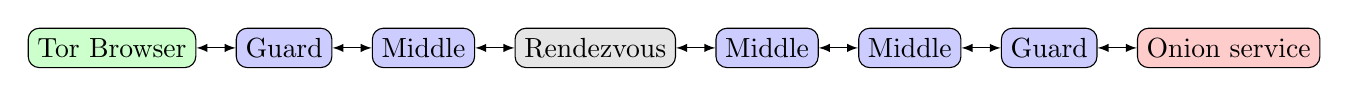
\begin{tikzpicture}[node distance=0.5cm]
\tikzset{>=latex}

\tikzstyle{block} = [rectangle, draw, rounded corners, text centered,
                     minimum height=0.5cm]

\node[block,fill=green!20]             (TB)  {Tor Browser};
\node[block,fill=blue!20,right=of TB]  (GR1) {Guard};
\node[block,fill=blue!20,right=of GR1] (MR1) {Middle};
\node[block,fill=gray!20,right=of MR1] (R)   {Rendezvous};
\node[block,fill=blue!20,right=of R]   (MR2) {Middle};
\node[block,fill=blue!20,right=of MR2] (MR3) {Middle};
\node[block,fill=blue!20,right=of MR3] (GR2) {Guard};
\node[block,fill=red!20,right=of GR2]  (OS)  {Onion service};

\draw[<->] (TB.east)  -- (GR1.west);
\draw[<->] (GR1.east) -- (MR1.west);
\draw[<->] (MR1.east) -- (R.west);
\draw[<->] (R.east)   -- (MR2.west);
\draw[<->] (MR2.east) -- (MR3.west);
\draw[<->] (MR3.east) -- (GR2.west);
\draw[<->] (GR2.east) -- (OS.west);

\end{tikzpicture}
\caption{When a user connects to an onion service, there are six relays in
between her Tor Browser (on the left) and the onion service (on the right).}
\label{fig:onion-service}
\end{figure*}

To create an onion domain, a Tor client first generates an RSA key pair.  It
then computes the SHA-1 hash over the RSA public key, truncates it to 80 bits,
and encodes these 80 bits in Base32, resulting in sixteen characters, \eg,
\texttt{expyuzz4wqqyqhjn}.  Due to the domain being a function of the public
key, onion domains are self-authenticating, meaning that as long as a client has
the correct domain, it knows what public key to expect.  The downside is that
sixteen random characters are impractical to remember.  However, onion domains
can be made at least partially meaningful by repeatedly creating RSA keys until
the resulting domain contains a desired string.  These domains are referred to
as \emph{vanity onion domains}.  The longer the desired string, the more time it
takes to find a matching key pair.  In practice, onion service operators use
tools such as scallion~\cite{scallion} that parallelize the search for suitable
keys to speed up the process.  Vanity domains are used by several organizations
such as Facebook (\url{facebookcorewwwi.onion}), ProPublica
(\url{propub3r6espa33w.onion}), and the New York Times
(\url{nytimes3xbfgragh.onion}).

Onion services are private by default.  Once an onion service is created, it is
up to its operator to announce it to the public, \eg, by adding it to onion site
search engines such as Ahmia.\footnote{The search engine is available online at
\url{https://ahmia.fi}.}  The lack of a go-to service such as Google for
onion service discovery means that the community has devised various ways to
publish onion services; most importantly an array of search engines and curated
lists.


\section{Interview study}
\label{sec:interview-study}

We conducted a series of semi-structured interviews about the use of Tor
Browser and onion services to explore user experience outside the constraints
of our online survey, and to inform the creation of our survey---and vice versa
because we conducted more interviews after our survey ended.

\subsection{Method}

We developed a question set that served as the basis for each interview.  The
semi-structured nature of the interviews allowed us to deviate from our
questions, \eg, by asking follow-up questions.  Our question set began with
demographic information (gender, age range, occupation, country of residence,
and level of education), followed by information about online behavior, and
finally questions specific to Tor Browser and onion services.

\subsubsection{Recruitment}

We created a short pre-interview survey (see
Appendix~\ref{sec:interview-survey}) to select eligible subjects.  This survey
was advertised in a post on The Tor Project's blog~\cite{Winter2017a} and its
Twitter account.  Our selection process focused on laypeople and sought to
maximize cultural, gender, location, education, and age diversity.  We ended up
interviewing seventeen subjects whose demographic information is shown in
Table~\ref{tab:interviewees}.  In addition to our online screening, we
recruited participants in person at an Internet freedom event.

It is difficult to draw a uniform sample of Tor users to interview. We belive
that The Tor Project's blog and Twitter account are mainly read by users who
are particularly technical while many non-technical users may install Tor
Browser in a one-off process and then never read anything again.  To make
matters worse, due to Tor Browser's very nature as an anonymity tool, many
users value their privacy significantly more than the average Internet user,
making it difficult to have users trust us enough to talk about their browsing
habits.  We believe that our sample is biased towards more knowledgable and
technical users, but it also shows how diverse Tor's user base is.  Our
participants were human rights activists, legal professionals, writers,
artists, and journalists, just to name a few.

\begin{table*}[ht]
    \centering
    \begin{tabular}{l r r l r r l r r l r r}
    \toprule
    Age & \# & \% &
    Gender & \# & \% &
    Country of residence & \# & \% &
    Education & \# & \% \\
    \midrule
    18--25 & 2  & 11.8 & Female & 5  & 29.4 & Australia      & 1 & 5.9  & No degree     & 1  & 5.9 \\
    26--35 & 10 & 58.8 & Male   & 12 & 70.6 & Canada         & 5 & 29.4 & High school   & 3  & 17.7 \\
    36--45 & 4  & 23.5 &        &    &      & Colombia       & 1 & 5.9  & Graduate      & 3  & 17.7 \\
    46--55 & 1  & 5.9  &        &    &      & Germany        & 1 & 5.9  & Post graduate & 10 & 58.8 \\
           &    &      &        &    &      & India          & 1 & 5.9  & & & \\
           &    &      &        &    &      & Indonesia      & 1 & 5.9  & & & \\
           &    &      &        &    &      & Mexico         & 1 & 5.9  & & & \\
           &    &      &        &    &      & Netherlands    & 1 & 5.9  & & & \\
           &    &      &        &    &      & South Korea    & 1 & 5.9  & & & \\
           &    &      &        &    &      & United Kingdom & 2 & 11.8 & & & \\
           &    &      &        &    &      & U.S.A.         & 2 & 11.8 & & & \\
    \bottomrule
    \end{tabular}
    \caption{The distribution over gender, age, country of residence, and
    education for our seventeen interview subjects.}
    \label{tab:interviewees}
\end{table*}

\subsubsection{Procedure}

We conducted thirteen interviews in person and four interviews remotely; over
Skype, Signal, WhatsApp, and Jitsi---depending on what our interviewees felt
the most comfortable with.  For in-person interviews we asked our interviewees
to sign a consent form.  This was not practical for remote interviews, so we
sent the consent form in advance over email and asked for verbal consent before
the interview.  In all cases we explicitly asked for permission to record the
conversation.  All except two participants agreed to have the interview
recorded.  For these two interviews we took notes instead.  All interviews
concluded with a debriefing phase in which we asked if our participants had any
remaining questions.  Some were curious if technical explanations they provided
earlier were correct.  Finally, we offered our participants a gift card worth
20 USD as a token of appreciation.

Once all interviews were transcribed, we employed qualitative data coding to
analyze the transcripts.  Each interview transcript was coded by two members of
our team.  This process identified TODO themes, all listed in
Appendix~\ref{sec:coding-themes}.

\subsection{Research ethics}

The institutional review board (IRB) of Princeton University deemed our study
exempt from further review.\footnote{Our IRB protocol number is 8251.}  Before
each in-person interview we asked our subjects to sign a consent form.  This
was not practical for remote interviews, so we sought permission from our IRB
to use verbal instead of written consent.  In all interviews we explicitly
asked for permission to record the conversation, to which all but two
participants agreed.  In these two cases the interviewer took notes instead.
Finally, we made it clear that our participants could withdraw their consent at
any time.  Once we transcribed our interview recordings, we deleted the
original recordings.  We used the services of the company Rev to have our
recordings transcribed.  A mutually-signed non-disclosure agreement protected
the confidentiality of our data.

\subsection{Results}

\subsubsection{Advantages}

\begin{itemize}
    \item Better privacy and security
    \item Gives you control over your data
    \item Perceived feeling of safety
\end{itemize}

\subsubsection{Disadvantages}

\begin{itemize}
    \item Slow browsing
    \item 90s browsing experience
    \item CAPTCHAs
    \item Tor makes you stick out
    \item Harmful ``public image'' of Tor
\end{itemize}

\subsubsection{Threat model}

\begin{itemize}
    \item Advertising companies
\end{itemize}

\subsubsection{Onion services}

\begin{itemize}
    \item Some users feel safer, some less safe when using onion services
\end{itemize}

\subsubsection{Miscellaneous}

\begin{itemize}
    \item Briding cultural gaps
\end{itemize}


\section{Online survey}
\label{sec:online-survey}

Approximately one month after we conducted our first batch of interviews, we
launched an online survey.  After having begun to explore the topic in our
interviews, the purpose of this survey was to obtain a large and diverse number
of responses for a number of specific questions.  We incorporated some of the
preliminary interview data in our survey questions.

\subsection{Method}
\label{sec:survey-design}

We created our survey in Qualtrics because our institution had a subscription,
and it came with all the features that we deemed necessary.  We verified that an
out-of-the-box Tor Browser could correctly take the survey.  However, Qualtrics
requires JavaScript which is deactivated when Tor Browser is set to its highest
security setting.  A number of users complained about the reliance on JavaScript
in the comments of our recruitment blog post~\cite{Winter2017a}.

Our survey was only available in English, but we targeted an international
audience because there are cultural differences in security
behavior~\cite{Sawaya2017a}.  Ignoring these differences would cause us to
optimize Tor Browser's user experience for a predominantly Western audience,
which is problematic.

While we were developing the survey, we used cognitive pretesting (sometimes
also called cognitive interviewing) to improve the wording of our
questions~\cite{Collins2003a}.  Pretesting reveals if respondents \first
understand questions, \second understand questions consistently, and \third
understand questions in the way that we intended.  In our pretests, we administered
our survey and asked the respondents to answer it while verbalizing their thought
process.  We occasionally asked follow-up questions to make sure that our
pretesters understood the questions as intended.  However, not all cognitive
processes can be verbalized, and cognitive pretesting may change the way
respondents answer questions.  We had five pretesters based on whose input we
iteratively improved our survey.  Two pretesters were native English speakers
while the remaining three were fluent but spoke English as a second language.

To weed out low-quality responses we incorporated four attention checks into our
survey~\cite{Berinsky2014a}.  Having four attention checks instead of just one
allows us to measure a respondent's \emph{degree} of attention, meaning that we
only discard responses that failed more than two attention checks.

The majority of our survey focused on onion services, but we also added some
questions about Tor in general.  Table~\ref{tab:survey-structure} shows that our
survey consists of six blocks that are ordered by topic.  It takes about fifteen
minutes to answer all questions.  The full survey is listed in
Appendix~\ref{app:interview-questions}.  Finally, we launched our survey on
August 16, 2017 and ended it on September 11, 2017, so it was active for 27
days.

\begin{table}[t]
	\centering
	\begin{tabular}{l r}
	\toprule
	Topic & \# of questions \\
	\midrule
	Consent and demographic information & 1 \\
	Tor usage & 4 \\
	Onion site usage & 20 \\
	Onion site operation & 5 \\
	Onion site phishing and impersonation & 9 \\
	Expectations of privacy & 9 \\
	End of survey & 1 \\
	\bottomrule
	\end{tabular}
	\caption{The topical question blocks in our survey and the number of
	questions they contain.}
	\label{tab:survey-structure}
\end{table}

\subsubsection{Recruitment}

Similar to our interviews, we advertised our survey in a blog post on The Tor
Project's blog~\cite{Winter2017a}, on its corresponding Twitter account, and on
three Reddit subforums.\footnote{The forums are \url{https://reddit.com/r/tor/},
\url{https://reddit.com/r/onions/}, and \url{https://reddit.com/r/samplesize/}.}
Again, note that this recruitment strategy is likely to bias our sample towards
more engaged users as casual Tor users are unlikely to follow The Tor Project's
blog or Twitter account.

\subsubsection{Research ethics}
Respondents had to agree to a consent form before starting the survey. The
consent form informed the respondents about the procedure of our experiment and
verified that all respondents were at least eighteen years of age.

To provide additional incentives, we originally planned to give respondents the
option to participate in a gift card lottery.  We abandoned the idea because it
was non-trivial to reconcile a lottery with anonymous participation because we
would have to collect our respondents' email addresses.  Despite the lack of
incentives, we collected a sufficient number of responses.  In fact, we believe
that many of our respondents were primarily motivated by improving Tor---some of
our interview participants turned down the gift cards that we offered.

\subsection{Results}
\label{sec:results}

Throughout all 27 days, our survey was taken 828 times.  However, not all
responses are necessarily of high quality; people may have rushed their answers,
aborted our survey prematurely, or given deliberately wrong answers.  We weed
out such low-quality responses that \first did not finish the survey and that
\second failed more than two out of our four attention checks.  We collected a
total of 828 responses but only 604 (73\%) completed the survey and 527 (64\%)
passed at least two attention checks.  The remainder of this section analyzes
these 527 responses.

Table~\ref{tab:survey-demo} shows the demographics of our survey.  Not
surprisingly, our respondents were \emph{young and educated}: more than sixty
percent are younger than 36, and another sixty percent have at least a graduate
degree.  Finally, another sixty percent consider themselves at least highly
knowledgeable in matters of Internet privacy and security.

\begin{table*}[t]
	\centering
	\begin{tabular}{l r l r l r l r}
	\toprule
	Gender & \% &
	Age & \% &
	Education & \% &
	Domain knowledge & \% \\
	\midrule
	Female & 8.9  & 18--25   & 35.5 & No degree     & 5.5  & No knowledge             & 0.5  \\
	Male   & 86.3 & 26--35   & 34.6 & High school   & 31.9 & Mildly knowledgeable     & 7.6  \\
	Other  & 4.8  & 36--45   & 17.5 & Graduate      & 42.3 & Moderately knowledgeable & 32.4 \\
	       &      & 46--55   & 8.7  & Post graduate & 20.4 & Highly knowledgeable     & 44.9 \\
	       &      & 56--65   & 2.5  &               &      & Expert                   & 14.6 \\
	       &      & $>$ 65   & 1.2  &               &      & & \\
	\bottomrule
	\end{tabular}
	\caption{The distribution over gender, age, education, and domain knowledge 
	for our 621 interview subjects.}
	\label{tab:survey-demo}
\end{table*}


\subsubsection{Biases}

As mentioned earlier, it is very difficult to draw a truly uniform sample of Tor
users.  The only way to reach all Tor users uniformly would be to modify Tor
Browser's landing page that is displayed on start.  Unfortunately, this approach
is very invasive.  We opted for asking The Tor Project to disseminate our survey
on its blog and social media accounts.  We believe that this recruitment
strategy came with the following biases.

\begin{description}
    \item[Survivor bias] We predominantly heard from people who can tolerate
        Tor's usability issues enough to still be around and take a survey on
        the topic.  We likely did not hear from many---if any---people who gave
        up on Tor and are no longer around to tell their tale.  The danger of
        survivor bias lies in optimizing the user experience for the subset of
        people who could tolerate a bad user experience.

    \item[Self-selection bias] Due to the nature of our online survey,
        participants could voluntarily select themselves into the group of
        respondents. \textbf{TODO}
        No paranoid people or people who don't like
        JavaScript.  Not a huge problem as we know how they think.  We also
        mostly reached people who are unusually engaged.
\end{description}

\subsubsection{Tor usage}

Our survey started with two general questions about the use of Tor Browser.
Figure~\ref{fig:tor-usage} illustrates how often our respondents use Tor
Browser.  Almost half of our participants use Tor Browser either daily or even
as their main browser.

Figure~\ref{fig:tor-threats} illustrates what entities our respondents seek to
protect themselves from when using Tor Browser.  The majority considers ad
companies, governments, and---most prominently---their ISP.  More relatable
entities such as family, employer, and school are less prevalent.

\begin{figure}[t]
    \centering
    \includegraphics[width=\linewidth]{figures/tor-usage.pdf}
    \caption{The usage frequency of Tor Browser among our respondents.  Almost
    half of our respondents use Tor Browser either daily or as their main
    browser.}
    \label{fig:tor-usage}
\end{figure}

\begin{figure}[t]
    \centering
    \includegraphics[width=\linewidth]{figures/tor-threats.pdf}
    \caption{The threat actors that our respondents seek to protect themselves
        from by using Tor Browser.}
    \label{fig:tor-threats}
\end{figure}

People who selected ``Other'' gave a variety of responses.  A number of
respondents specifically pointed out Google and Facebook.  ISPs, backbone ISPs,
and websites were another common theme.  A number of respondents are struggling
with personal threats that include identity theft, targeted harassment, and
stalking.  Research is another common theme: Several respondents want to learn
about a topic without revealing their interest in it.  Some respondents use Tor
for search engine optimization, computer security research, and to research
medical conditions.  Finally, Tor provides technical advantages that don't
involve a threat actor.  Some respondents want IPv6 connectivity, evasion of
geographical content restrictions, and access to onion services.  A small number
of respondents are only interested in technical aspects other than privacy.  One
respondent stated that they don't need anonymity themselves but instead use Tor
to provide cover traffic for ``people who need protection.''

\subsubsection{Onion service usage}

The usage frequency of onion services is almost uniformly distributed among our
respondents; 24\% use onion sites less than once a month, 22\% use them about
monthly, 25\% weekly, and 23\% daily.  The remaining 6\% has never used an onion
service before.

The majority of our respondents (61.8\%) has used onion services for purposes
other than web browsing before.  Several protocols such as the chat application
Ricochet~\cite{ricochet} and the file sharing application
OnionShare~\cite{onionshare} were purpose-built on top of onion services while
existing TCP-based tools such as SSH can also be used with onion addresses
instead of traditional IP addresses.  Almost one third (29.7\%) of our
participants use onion service for non-browsing activities at least once a week.

But why do Tor users browse onion services in the first place?
Figure~\ref{fig:onion-usage} provides an answer.  The majority uses onion
services because of the additional anonymity (70\%) and the additional security
(61\%).  For 46\% it is the only way to access some content they enjoy, so using
onion services is a necessity.  27\% of our respondents found themselves curious
about the ``Dark Web'' and set out to find their own answer and 19\%
occasionally stumble upon links to onion services in their day-to-day browsing
activity.  Respondents who selected ``Other'' gave a variety of reasons, the
most predominant of which was the ability to set up a TCP service behind a NAT
device.  That way, it is possible to run an SSH server in a home network that
has neither a permanent IP address, nor port forwarding.  Other noteworthy
respondents use onion services to reduce the load on exit relays, to do
technical research, and to access sites that are otherwise unavailable.

\begin{figure}[t]
    \centering
    \includegraphics[width=\linewidth]{figures/onion-usage.pdf}
    \caption{Our respondents' (multiple choice) reasons for using onion
    services.}
    \label{fig:onion-usage}
\end{figure}

\subsubsection{Onion service discovery}

Recall that onion services are private by default, leaving it up to their
operator to disseminate the domain.  Established search engines such as Google
are therefore inadequate to find content on onion services.  We wanted to find
out how our respondents discover onion services.
Figure~\ref{fig:onion-discovery} illustrates the results.  The three most
popular ways of discovering new onion sites, all approximating 50\%, are social
networking sites such as Twitter and Reddit, the list of search engines such as
Ahmia\footnote{Ahmia.fi is an onion site search engine that crawls
user-submitted onion domains.  It publishes the list of all indexed onion
services at \url{https://ahmia.fi/onions/}.}, and randomly encountering links
when browsing the web.

While significantly less popular, discovering onion domains through friends and
family has the advantage of trust.  Some of our interview participant indicated
that they heavily rely on this distribution method simply because they can trust
the origin.  Finally, a mere 4\% indicated that they are not interested in
learning about new onion services.

Respondents who selected ``Other'' predominantly brought up
independently-maintained lists of onion services and aggregators.  A noteworthy
example is the Hidden Wiki.

\begin{figure}[t]
    \centering
    \includegraphics[width=\linewidth]{figures/onion-discovery.pdf}
    \caption{Our respondents' (multiple choice) methods of discovering onion
    services.}
    \label{fig:onion-discovery}
\end{figure}

The next question in our survey then asked if our respondents are satisfied with
the way they discover onion services.  60\% selected ``Yes'' while 40\% selected
``No.'' Some respondents who selected ``Yes'' brought up that they have no
interest in learning about new onion services, in part because they only use a
small set of onion services.  Among the people who are not satisfied, the most
prominent complaint was about broken links on onion site lists.  There is
non-trivial churn among onion sites and our respondents were frustrated that
existing lists are typically not curated and contain many dead links.

Many respondents were not aware of search engines such as ahmia.fi.  Among those
that were, many were not satisfied with both the search results and the number
of indexed onion sites.  Unsurprisingly, a ``Google for onion sites'' was a
frequent wish.

Several respondents were unhappy with existing aggregators.  In addition to
broken links, some distrust lists because they occasionally contain scam and
phishing sites.  The difficulty of telling apart two given onion domain names
exacerbates this issue.  Another common wish for aggregators was for them to be
more verbose in their description of onion sites.  In particular, some
respondents want to avoid illegal and pornographic content, which is often
difficult if the description is vague and the onion domain reveals nothing about
its content.

Many respondents expressed frustration about the difficulty of finding out if
site X also provides a corresponding onion service.  A common wish was to have
site X list its onion service prominently in a footer.  Ironically, some
respondents were surprised that torproject.org has a corresponding onion site --
they couldn't find it on the web site.

Interestingly, some respondents voiced frustration about various usability
issues, but mentioned in the same sentence that this is an inherent trade-off of
privacy technology, suggesting that there is nothing that can be done about it.

\subsubsection{Onion service domain format}

Conventional domains are designed to be easy to remember and recognize.  But how do users
handle the randomly-generated onion domains?  Question 3.8 in our survey asked
exactly that, with the responses being illustrated in
Figure~\ref{fig:onion-domain-mgmt}.

\begin{figure}[t]
    \centering
    \includegraphics[width=\linewidth]{figures/onion-domain-mgmt.pdf}
    \caption{The strategies that our respondents use to handle onion domains.
    More than half use bookmarks inside of Tor Browser and a quarter thinks that
    there's no good solution.}
    \label{fig:onion-domain-mgmt}
\end{figure}

Most respondents use bookmarks inside Tor Browser for onion domains.  While
convenient, it leaves a trace of (presumably) visited sites on one's computer.
One of Tor Browser's security requirements is ``disk avoidance,'' \ie, the
browser must not write anything to disk that would reveal the user's browsing
history~\cite[\S~2.1]{Perry2017a}.  Bookmarking links is a violation of this
security requirement.  Many of our respondents were aware of this issue.  About
a dozen respondents who selected ``Other'' stated that they store onion domains
encryptedly---either in a text file or in their password manager.

Somewhat less popular is saving onion domains in local text files (36\%),
getting them from trusted websites (34\%), use search engines (18\%), memorize
domains (16\%), use some other techniques (9\%) or employ pen and paper (8\%).
Notably, one quarter of our respondents does not have a good solution to the
problem.  Given the alarming number of (possibly insecure) home-baked solutions,
a Tor Browser extension may be warranted to approach the problem.

The next question in our survey asked if our respondents expect the
next-generation domain format to change their browsing habits.  Interestingly,
only 17\% expect to have their browsing habits changed while 83\% don't.  Among
the respondents who selected ``Yes,'' many expressed that they memorize a small
number of onion domains (such as Facebook's), which will no longer be possible.
People who selected ``No'' mostly bring up that they treat onion domains as
opaque identifiers that they handle via tools such as bookmarks.  These results
suggest that the current state is dire, yet not expected to get much worse with
the new domain format.

Problematic:
``I only memorize the first part of the domain''

``If there isn't some cognizable word at the start, it'll be more difficult for
me to determine if I'm going to the correct domain or a scam. I may end up going
to less .onion sites as a result.''

\subsubsection{Onion service operation}

A survey question block on onion service operation shed light on the reasons for
running onion services and what sort of issues users face when doing so.  40\%
of our respondents once set up an onion service.  Among the respondents who
never have, 31\% have considered doing so while 30\% have never even considered
it.  Interestingly, 79\% of operators have run an onion service for private use
while 53\% have run them for the public.

Figure~\ref{fig:onion-operation-reasons} gives an overview of the reasons for
running onion services.  Interestingly, the extra security properties overshadow
the anonymity properties of onion services.  Another particularly popular reason
is NAT traversal---many respondents noted that onion services allow them to
expose a TCP service in their home network despite being behind a NAT device.
Finally, some people run onion service indirectly because third-party tools such
as OnionShare~\cite{onionshare} or Ricochet~\cite{ricochet} are built on top of
them.  Onion services can have clear benefits for businesses as well as
evidenced by one respondent who wrote on onion services: ``We use it for
delivering updates to our router to customers securely and without leaking
metadata.''

\begin{figure}[t]
    \centering
    \includegraphics[width=\linewidth]{figures/onion-operation-reasons.pdf}
    \caption{The reasons people have for running onion services.}
    \label{fig:onion-operation-reasons}
\end{figure}

Figure~\ref{fig:onion-operation-concerns} illustrates the concerns that onion
service operators face.  We consider three attacks; \first somebody setting up a
phishing site for the operator's site, \second a denial-of-service attack, and
\third a deanonymization attack.  More than half of our respondents are at least
somewhat concerned about all of these attacks.  Almost 40\% claim to be
extremely concerned about somebody deanonymizing their onion service.  Indeed,
many respondents lamented the difficulty of knowing that an onion service setup
is robust against application-layer deanonymization attacks.

\begin{figure}[t]
    \centering
    \includegraphics[width=\linewidth]{figures/onion-operation-concerns.pdf}
    \caption{The level of concern onion service operators have with respect to a
    phishing clone of their service, denial-of-service attacks, and
    deanonymization.}
    \label{fig:onion-operation-concerns}
\end{figure}

\subsubsection{Susceptibility to phishing}
\begin{itemize}
    \item Attack partially documented in academic
        literature~\cite[\S~5.1]{Winter2016a}.  Monteiro provided a
        timeline~\cite{Monteiro2016a}.
    \item Many ad-hoc anti-phishing methods, some of which incorrect.
\end{itemize}

\subsubsection{Perception of vanity onion domains}
\begin{description}
    \item[$+$] Combination of vanity prefix and Markov Model-selected suffix can
        deliver memorable domain for v2 domains.
    \item[$+$] Reveals what the onion service is hosting.
    \item[$-$] May provide false sense of security.
    \item[$-$] Only available to people with resources.
    \item[$-$] Conflicts with people's (flawed) expectation that a domain must
        be random to stay hidden.
\end{description}

Technical ways to exacerbate creation of vanity domains: Incorporate scrypt into
key generation process.
If vanity domains remain, have Tor process support it?


\section{Discussion}
\label{sec:discussion}

\subsection{Biases}

It is difficult to draw a truly uniform sample of Tor users.  The only way to
reach all Tor users uniformly would be to modify Tor Browser's landing page
that is displayed on start---an approach that we considered prohibitively
invasive.  Instead, we decided to ask The Tor Project to disseminate our survey
on its blog and social media accounts.  We believe that this recruitment
strategy was subject to the following biases.

\paragraph{Non-response bias.} 
People who noticed our call for volunteers and decided against participating
may exhibit traits that are fundamentally different from those who did
participate.  These non-respondents may have valued their privacy too much,
falsely believed that their experience is irrelevant, lacked the time, or had
other reasons not to participate.

\paragraph{Survivor bias.}
We predominantly heard from people who can tolerate Tor's usability issues,
which is why they are still around to tell their tale.  We likely did not hear
from many---if any---people who gave up on Tor and were thus unable to tell us
what drove them away.  The danger of survivor bias lies in optimizing the user
experience for the subset of people who can tolerate a non-optimal user
experience.

\paragraph{Self-selection bias.}
Due to the nature of our online survey, participants could voluntarily select
themselves into the group of respondents.  This set of people may be unusually
engaged and technical, which is why they have formed opinions that they
consider worth sharing.

\subsection{Take-aways for Tor developers}

Several of our interview participants pointed out Tor Browser's antiquated user
interface.  Past work has shown that users interpret unrelated aspects such as
voice quality as a proxy signal for security, which raises the question if the
same holds true for user interface design~\cite[\S~IV.A]{Abu-Salma2017a}.  If
so, it is important to equip Tor Browser with a modern user interface.

\begin{figure}[t]
    \centering
    \includegraphics[width=\linewidth]{figures/tor-comic.jpg}
    \caption{A comic draft that illustrates what Tor can and cannot provide for
        non-technical users.  The comic was drawn by artist Jason Li while
        working with one of the authors.}
    \label{fig:tor-comic}
\end{figure}

\subsection{Take-aways for Tor users}

The strong security properties of onion services are futile if users cannot tell
apart a genuine domain from its impersonation.  Awareness of this issue is the
first step and several onion services have long begun to alert their users.



% could tor show you when an onion service descriptor was first published?


\subsection{Take-aways for Tor researchers}

We found it challenging, yet rewarding and illuminating to study the Tor
community.  Tor users obviously value their privacy which reduces their
willingness to participate in research projects.  Past academic research
projects that involved questionable methods turned this care into distrust for
many users.  Showing willingness to directly interact with the community and
taking seriously their concerns signals respect and transparent methods.  For
our online survey, we recommend to use software that works in Tor
Browser\footnote{Note that Tor Browser supports three security levels; the
default of ``low,'' ``medium,'' and ``high.''  Some users brought to our
attention that our survey did not work when the security level is set to
``high'' because it disables JavaScript, which our survey required---an
oversight on our end.} and does not fetch tracking scripts such as Google
Analytics.  For the survey design, one likely has to forego asking questions
that are best practice such as income level and country of residence.  We made
even the basic information we asked optional so our respondents had the chance
to answer the survey without providing any personal information at all.  In our
interviews we tried to accomodate the needs of our participants by using
software of their choice.


\section{Conclusion}
\label{sec:conclusion}

In this work we studied how Tor users interact with onion services and the
broader technology that enables onion services.  Drawing on a mixed-methods
approach, we conducted seventeen semi-structured interviews and collected 828
responses to our online survey.  These two data sets served as the basis of our
analysis and provided unique insight into how Tor users perceive, use, and
understand Tor in general and onion services in particular.

We find that the current state of onion services resembles the web of the 90s.
Pages load slowly, user interfaces are clumsy, and search engines fall short of
expectations.  Users appreciate the extra security, privacy, and \textsc{nat}
punching properties of onion services, giving rise to numerous use cases, but
are frequently wary of the content that is hosted on them.  Some users found
ways to manage what is perhaps the most striking idiosyncracy of onion
services---their domain format---by using bookmarks, (encrypted) files
containing links, and referring to trusted link aggregators.  Many users however
have flawed mental models of onion services that could increase their
susceptibility to phishing attacks.

Our code, data, and auxiliary resources are available on our project page at
\url{https://nymity.ch/onion-services/}.


\section*{Acknowledgements}
We want to thank George Kadianakis for helpful feedback.

We want to thank Laura M. Roberts, Roya Ensafi, Will Scott, and Jens Kubiziel
for help with pre-testing the survey.

Thanks to Katherine Haenschen for helping us improve our method.

This research was supported in part by the Center for Information Technology
Policy at Princeton University.  This project was further supported in part by
National Science Foundation Awards CNS-1540055 and CNS-1602399.


\balance

{\footnotesize
\printbibliography}

\appendix

\section{Pre-interview survey}
\label{app:interview-survey}
We asked potential interview subjects to fill out a short survey (see below)
before we proceeded with selecting our subjects.  This survey allowed us to
select for subjects with the most interesting background.

\begin{enumerate}
    \item What is your name?
    \item What is your email address?
    \item Are you 18 years or older?
        \begin{itemize}[label=$\Circle$]
            \item Yes
            \item No
        \end{itemize}
    \item Have you used Tor Browser in the past?
        \begin{itemize}[label=$\Circle$]
            \item Yes
            \item No
        \end{itemize}
    \item Have you used onion services in the past?
        \begin{itemize}[label=$\Circle$]
            \item Yes
            \item No
        \end{itemize}
    \item How do you rate your knowledge about Internet privacy and security?
        \begin{itemize}[label=$\Circle$]
            \item Not at all knowledgeable
            \item Slightly knowledgeable
            \item Somewhat knowledgeable
            \item Moderately knowledgeable
            \item Extremely knowledgeable
        \end{itemize}
\end{enumerate}

\section{Interview questions}
\label{app:interview-questions}

We started the interview by handing our interviewees the consent form and
explained the purpose of our research to them.

\paragraph{Introductory questions}
\begin{enumerate}
    \item Tell us how often and why you use Tor?
    \item Do you remember the first time you used Tor?
\end{enumerate}

\paragraph{Expectations of privacy}
\begin{enumerate}
    \item What would make you use onion services more? (speed, quality/quantity
        of content, better domain format, popular websites having onion sites)
    \item Who or what are you trying to protect yourself against when using Tor?
    \item The domain format of onion sites is weird.  How do you deal with that?
    \item Would you like it if Tor Browser automatically redirected you to onion
        sites?  Even if that were the case for all onion sites?
    \item How do you learn about new onion sites?
    \item Do you think phishing is a concern with onion sites?  How do you know
        if an onion site is legitimate?
    \item Assume you use Tor to open \texttt{example.com}.  Who can see what?
        What if you open the corresponding onion site instead?
    \item What are you concerned about when using Tor?
    \item Certain things are hidden from certain entities when you are using
        Tor.  Please explain your beliefs.
    \item Some websites use ``vanity onion domains.''  Whare are your thoughts
        on that?
    \item Explain in your own words how you believe Tor works.
    \item Is there anything else about the usability of onion services that you
        wish to share?
\end{enumerate}

\section{Survey questions}
This section contains our online survey, consisting of seven sections.  Each
section holds a number of questions and their respective responses.  In the
responses, circles indicate that only one response can be selected while squares
indicate the possibility to select multiple responses.

\subsection{Demographic information}
\begin{enumerate}
    \item What is your gender?
        \begin{itemize}[label=$\Circle$]
            \item Female
            \item Male
            \item Other
        \end{itemize}

    \item What is your age?
        \begin{itemize}[label=$\Circle$]
            \item 18--25 years
            \item 26--35 years
            \item 36--45 years
            \item 46--55 years
            \item 56--65 years
            \item Older than 65 years
        \end{itemize}

    \item What is the highest level of education that you completed?
        \begin{itemize}[label=$\Circle$]
            \item Some education, but no high school diploma or equivalent
            \item High school diploma or equivalent
            \item College or university degree (for example a bachelor's degree)
            \item Post-graduate education (for example a master's or a doctorate degree)
        \end{itemize}

    \item How would you rate your knowledge about Internet privacy and security?
        \begin{itemize}[label=$\Circle$]
            \item No knowledge
            \item Mildly knowledgeable
            \item Moderately knowledgeable
            \item Highly knowledgeable
            \item Expert
        \end{itemize}
\end{enumerate}

\subsection{Tor usage}
\begin{enumerate}
    \item Tor Browser is a web browser---similar to Firefox---that allows you
        to browse the web anonymously. Have you ever used Tor Browser?
        \begin{itemize}[label=$\Circle$]
            \item Yes
            \item No
        \end{itemize}

    \item How frequently do you use Tor Browser?\\(Please select the answer
        that applies the most.)
        \begin{itemize}[label=$\Circle$]
            \item Never
            \item On average less than once a month
            \item On average about once a month
            \item On average about once a week
            \item On average about once a day
            \item Tor Browser is my main browser
        \end{itemize}

    \item When using Tor Browser, who do you want to protect your browsing
        activity from?\\(Check all that apply.)
        \begin{itemize}[label=$\Square$]
            \item My government
            \item Other governments
            \item My Internet service provider (ISP)
            \item My school
            \item My employer
            \item Friends and family
            \item Advertising companies
            \item Hackers in open WiFis (for example in coffee shops)
            \item Other (Please elaborate below.)
        \end{itemize}

    \item For quality purposes, please select only ``iPhone'' and ``Android''
        in the options below.
        \begin{itemize}[label=$\Square$]
            \item PC
            \item Mac
            \item iPhone
            \item Android
            \item Other (Please elaborate below.)
        \end{itemize}
\end{enumerate}

\subsection{Onion site usage}
\begin{enumerate}
    \item The Tor Browser allows you to browse ``onion sites.'' Onion sites are
        web sites that can only be accessed over the Tor network. The domains of
        onion sites end with \texttt{.onion} instead of \texttt{.com},
        \texttt{.net}, etc.; they are of constant length; and they tend to
        ``look random.'' For example, The Tor Project's web site,
        \texttt{torproject.org}, is also available at
        \texttt{expyuzz4wqqyqhjn.onion} as an onion site.

    \item How frequently do you use Tor Browser to browse onion sites?\\(Please
        select the answer that applies the most.)
        \begin{itemize}[label=$\Circle$]
            \item I have never used onion sites
            \item On average less than once a month
            \item On average about once a month
            \item On average about once a week
            \item On average about once a day
        \end{itemize}

    \item How frequently do you use onion sites for purposes other than web
        browsing? For example for remote login (SSH) or chat (IRC, or XMPP)?
        \begin{itemize}[label=$\Circle$]
            \item Never
            \item On average less than once a month
            \item On average about once a month
            \item On average about once a week
            \item On average about once a day
        \end{itemize}

    \item Why do you browse onion sites?\\(Check all that apply.)
        \begin{itemize}[label=$\Square$]
            \item Because of the additional anonymity -- traffic to onion sites
                never leaves the Tor network
            \item Because of the additional security -- onion sites provide
                end-to-end security
            \item Some sites I like are only available as onion sites and not
                as normal web sites
            \item No particular reason; I occasionally just click on links to
                onion sites
            \item I read about the ``dark web'' and wanted to form my own
                opinion
            \item Other (Please elaborate below.)
        \end{itemize}

    \item How do you discover new onion sites?\\(Check all that apply.)
        \begin{itemize}[label=$\Square$]
            \item I browse the list of onion site search engines such as
                \texttt{ahmia.fi}
            \item From social networking sites such as Reddit or Twitter
            \item Recommendations from friends and family
            \item I randomly encounter them while browsing the web
            \item I am not interested in learning about new onion sites
            \item Other (Please elaborate below.)
        \end{itemize}

    \item Are you satisfied with the way you discover new onion sites?\\(Check
        all that apply.)
        \begin{itemize}[label=$\Circle$]
            \item Yes
            \item No (Please elaborate below.)
        \end{itemize}

    \item Many people memorize popular domains such as \texttt{youtube.com} and
        \texttt{wikipedia.com} for quick access. How do you deal with the domain
        of onion sites such as \texttt{expyuzz4wqqyqhjn.onion}?\\(Check all that
        apply.)
        \begin{itemize}[label=$\Square$]
            \item I save a list of onion domains in a file on my computer
            \item I write onion domains down using pen and paper
            \item I bookmark onion domains in Tor Browser
            \item I use a web-based bookmarking service such as Firefox Sync or
                Google Bookmarks
            \item I use a search engine each time (for example, to search for
                ``facebook onion site'')
            \item I go to web pages I trust that have links to onion sites
            \item I memorize some onion domains
            \item I don't have a good solution
            \item Other (Please elaborate below.)
        \end{itemize}

    \item The Tor Project is currently working on the next generation of onion
        services. The new onion domain format will consist of 52 characters,
        for example:
        \texttt{a1uik0w1gmfq3i5ievxdm9ceu27e88g6o7pe0rffdw9jmn\-twkdsd.onion}
        Do you expect this to change your browsing habits?
        \begin{itemize}[label=$\Circle$]
            \item Yes (Please elaborate below.)
            \item No (Please elaborate below.)
        \end{itemize}

    \item Do you have a Facebook account?
        \begin{itemize}[label=$\Circle$]
            \item Yes
            \item No
        \end{itemize}

    \item Have you ever logged in to Facebook over its onion site
        \texttt{facebookcorewwwi.onion}?
        \begin{itemize}[label=$\Circle$]
            \item Yes, that is the only way I log in to Facebook
            \item Yes, occasionally
            \item No, never
            \item I didn't know about this onion site until now
        \end{itemize}

    \item For quality purposes, please select ``Yes, more than once'' in the
        options below.
        \begin{itemize}[label=$\Circle$]
            \item Yes, once
            \item Yes, more than once
            \item No
        \end{itemize}

    \item How many onion domains do you have fully memorized?
        \begin{itemize}[label=$\Circle$]
            \item None
            \item One
            \item Two
            \item Three
            \item Four
            \item More than four
        \end{itemize}

    \item Is \texttt{facebookcorewwwi.onion} among the sites that you have
        memorized?
        \begin{itemize}[label=$\Circle$]
            \item Yes
            \item No
        \end{itemize}

    \item Why do you memorize onion domains?\\(Check all that apply.)
        \begin{itemize}[label=$\Square$]
            \item It allows me to open the site more quickly
            \item I don't want to leave any digital traces of the onion sites I
                visit
            \item That way I can be sure that I end up at the right onion site
                and not a phishing site
            \item After typing a domain many times, I automatically start to
                memorize it
            \item Other (Please elaborate below.)
        \end{itemize}

    \item Imagine you had to memorize onion domains. Please rate the difficulty
        of memorizing the following domains.
        \begin{itemize}
            \item \texttt{facebookcorewwwi.onion}
            \item \texttt{expyuzz4wqqyqhjn.onion}
            \item \texttt{torproz4wqqyqhjn.onion}
            \item \texttt{torprojectqyqhjn.onion}
        \end{itemize}
        For each answer, we provided the following Likert scale:
        \begin{itemize}
            \item Very easy
            \item Somewhat easy
            \item Neither easy nor difficult
            \item Somewhat difficult
            \item Very difficult
        \end{itemize}

    \item Please explain the reason for the rating you gave above.

    \item If popular web sites such as YouTube, Twitter, or Amazon offered
        onion sites in parallel to their normal web sites, which one would you
        prefer?
        \begin{itemize}[label=$\Circle$]
            \item Always the normal web site
            \item Always the onion site
            \item Other (Please elaborate below.)
        \end{itemize}

    \item Please explain the reason for the choice you made above.

    \item If Tor Browser could automatically redirect you from a web site to
        its corresponding onion site (for example from \texttt{facebook.com} to
        \texttt{facebookcorewwwi.onion}), would you use this feature?
        \begin{itemize}[label=$\Circle$]
            \item No, never
            \item Yes, for some sites
            \item Yes, always
            \item Other (Please elaborate below.)
        \end{itemize}

    \item Please explain the reason for the choice you made above.

    \item Please rate how important the following criteria are for the
        usability of onion sites.\\(Check all that apply.)
        \begin{itemize}
            \item Page load time
            \item Quality of content (e.g., up-to-date, interesting sites)
            \item Diversity of content (e.g., sites about politics, technology, social media, etc.)
            \item Easy-to-remember domain format
            \item Having an onion service version of popular services such as Facebook
            \item Existence of a search engine (like Google) for onion services
        \end{itemize}
        For each answer, we provided the following Likert scale:
        \begin{itemize}
            \item Very unimportant
            \item Somewhat unimportant
            \item Neutral
            \item Somewhat important
            \item Very important
        \end{itemize}
\end{enumerate}

\subsection{Onion site operation}
\begin{enumerate}
    \item Have you ever set up your own onion site?
        \begin{itemize}[label=$\Circle$]
            \item Yes
            \item No, but I have considered doing it
            \item No, and I have not considered it
        \end{itemize}

    \item Did you experience any issues while setting up your onion site?
        \begin{itemize}[label=$\Circle$]
            \item No
            \item Yes (Please elaborate below.)
        \end{itemize}

    \item Why did you set up your own onion site?\\(Check all that apply.)
        \begin{itemize}[label=$\Square$]
            \item I wanted my site to be anonymous
            \item I wanted my site to have end-to-end security
            \item I used a tool that automatically creates onion sites (for
                example OnionShare or Ricochet)
            \item To make my site accessible behind a NAT device
            \item Out of curiosity
            \item Other (Please elaborate below.)
        \end{itemize}

    \item Were the onion site(s) you set up intended for the general public, or
        only for private use?\\(Check all that apply.)
        \begin{itemize}[label=$\Square$]
            \item For public use (for example, a public blog)
            \item For private use (for example, sharing pictures with a friend)
        \end{itemize}

    \item Please rate the level of concern you would have for the following
        scenarios.
        \begin{itemize}
            \item Somebody deanonymizing my onion service
            \item Somebody taking my onion service offline
            \item Somebody setting up a phishing site targeting my onion service
        \end{itemize}
        For each answer, we provided the following Likert scale:
        \begin{itemize}
            \item Not at all concerned
            \item Slightly concerned
            \item Somewhat concerned
            \item Moderately concerned
            \item Extremely concerned
        \end{itemize}
\end{enumerate}

\subsection{Onion site phishing and impersonation}
\begin{enumerate}
    \item Did you ever type an onion domain manually?
        \begin{itemize}[label=$\Circle$]
            \item Yes
            \item No
        \end{itemize}

    \item Please elaborate on why you typed an onion domain manually?

    \item How do you realize that you made a typo when typing an onion
        URL?\\(Check all that apply.)
        \begin{itemize}[label=$\Square$]
            \item When the page won't load
            \item When a wrong page shows up
            \item I don't know
            \item Other (Please elaborate below.)
        \end{itemize}

    \item Have you ever thought about whether the onion site you are browsing
        is the authentic site you are trying to reach?
        \begin{itemize}[label=$\Circle$]
            \item Yes
            \item No
        \end{itemize}

    \item How do you know an onion site is the legitimate site you are trying
        to reach, and not an impersonation?\\(Check all that apply.)
        \begin{itemize}[label=$\Square$]
            \item I verify (part of) the onion domain in Tor Browser's address
                bar
            \item I use bookmarks when accessing onion sites
            \item I go to the corresponding web site and look for the link to
                its onion site
            \item Sometimes I cannot tell the difference between the legitimate
                and the impersonation site
            \item I copy\&paste onion domains from a trusted source
            \item I check if the onion site's HTTPS certificate is valid (if it
                has one)
            \item I don't check
            \item Other (Please elaborate below.)
        \end{itemize}

    \item How many characters of a domain do you verify? Recall that an onion
        domain has 16 characters.
        \begin{itemize}[label=$\Circle$]
            \item 1--3
            \item 4--6
            \item 7--9
            \item 10--12
            \item 13--16
        \end{itemize}

    \item For quality purposes, please select ``Less than once a month'' in the
        options below.
        \begin{itemize}[label=$\Circle$]
            \item Less than once a month
            \item About once a month
            \item About once a week
            \item About once a day
        \end{itemize}

    \item Have you ever sent Bitcoins to a Bitcoin address that you got from an
        onion site?
        \begin{itemize}[label=$\Circle$]
            \item Yes
            \item No
        \end{itemize}

    \item Some onion site owners use tools to have a short word at the
        beginning of their onion domain. This is why Facebook's domain
        (\texttt{facebookcorewwwi.onion}) looks the way it does. We call these
        customized domains ``vanity onion domains.''

    \item What is your overall opinion on vanity onion domains?\\(Check all
        that apply.)
        \begin{itemize}[label=$\Square$]
            \item I find them useful because they are easier to memorize
            \item I find them useful because they are easier to recognize
            \item I like them because they make an onion site look ``unique''
            \item I dislike them because onion sites shouldn't contain their
                name in their domain
            \item I don't see a benefit
            \item I don't have an opinion
            \item Other (Please elaborate below.)
        \end{itemize}
\end{enumerate}

\subsection{Expectations of privacy}
\begin{enumerate}
    \item Let us move away from onion services and turn to expectations of
        privacy. If you use Tor Browser to open \texttt{http://example.com}, who
        do you believe can see your connection to
        \texttt{http://example.com}?\\(Check all that apply.)
        \begin{itemize}[label=$\Square$]
            \item Your Internet service provider (ISP)
            \item The ISP of \texttt{example.com}
            \item Your Tor ``exit relay''
            \item Your Tor ``guard relay''
            \item Nobody
            \item I don't know
            \item Other (Please elaborate below.)
        \end{itemize}

    \item Now imagine that you are instead using Tor Browser to open the
        \emph{onion site} of \texttt{http://example.com}. Who do you believe can
        see your connection to this onion site?\\(Check all that apply.)
        \begin{itemize}[label=$\Square$]
            \item Your Internet service provider (ISP)
            \item The ISP of the onion site
            \item Your Tor ``exit relay''
            \item Your Tor ``guard relay''
            \item The ``guard relay'' of the onion site
            \item Nobody
            \item I don't know
            \item Other (Please elaborate below.)
        \end{itemize}

    \item How safe do you feel when using Tor Browser compared to another
        browser?
        \begin{itemize}[label=$\Circle$]
            \item Very unsafe
            \item Somewhat unsafe
            \item Neutral
            \item Somewhat safe
            \item Very safe
        \end{itemize}

    \item Please elaborate on why you feel that way when using Tor Browser.

    \item Please tell us about how safe you feel when browing onion sites as
        compared to normal websites?
        \begin{itemize}[label=$\Circle$]
            \item Very unsafe
            \item Somewhat unsafe
            \item Neutral
            \item Somewhat safe
            \item Very safe
        \end{itemize}

    \item Please elaborate on why you feel that way when using onion sites.

    \item For quality purposes, please select only ``Very unsafe'' in the options
        below.
        \begin{itemize}[label=$\Circle$]
            \item Very unsafe
            \item Somewhat unsafe
            \item Neutral
            \item Somewhat safe
            \item Very safe
        \end{itemize}

    \item Assume you just set up your own onion site. Who do you believe can
        see that this onion site was set up?\\(Check all that apply.)
        \begin{itemize}[label=$\Square$]
            \item The onion site's ISP
            \item The developers of The Tor Project
            \item (Some) Tor relays
            \item Nobody
            \item I don't know
            \item Other (Please elaborate below.)
        \end{itemize}

    \item Facebook already runs the onion site \texttt{facebookcorewwwi.onion}.
        How difficult or easy do you believe is it for someone to create domains
        that begin with the following characters? Note that the {\color{red}
        \texttt{X}} symbols below
        are just placeholders. What matters is the first characters.
        \begin{itemize}
            \item \texttt{facebookcore\textcolor{red}{XXXX}.onion}
            \item \texttt{facebook\textcolor{red}{XXXXXXXX}.onion}
            \item \texttt{face\textcolor{red}{XXXXXXXXXXXX}.onion}
        \end{itemize}
        For each answer, we provided the following Likert scale:
        \begin{itemize}
            \item Very easy
            \item Moderately easy
            \item Neither easy nor difficult
            \item Moderately difficult
            \item Very difficult
            \item I don't know
        \end{itemize}
\end{enumerate}

\subsection{End of survey}
\begin{enumerate}
    \item Finally, is there anything else about the usability of Tor or onion
        services that you wish to share with us?
\end{enumerate}


\end{document}
